\documentclass[a4paper,12pt]{report}
\usepackage[utf8]{inputenc}
\usepackage{enumitem} %permite el uso de letras para enumerar
\usepackage{graphicx} %para las imágenes
\usepackage{float} %para fijar las imágenes

\usepackage{tikz}
\usetikzlibrary{arrows.meta, positioning} %para hacer diagramas de bloques

\usepackage{amsmath}%para entornos de alineación
\usepackage{amsfonts}%para las letras lindas de matemática
\usepackage{xfrac}%para fracciones chiquitas
\setlength{\jot}{8pt}%modifica el interlineado

\usepackage{tikz} %Librería para gráficos
\usetikzlibrary{calc, arrows.meta, positioning}

\usepackage[a4paper, %margenes de pagina
  left=2.5cm,
  right=2.5cm,
  top=2cm,
  bottom=2cm,
  includehead
]{geometry}

\usepackage{fancyhdr}
\pagestyle{fancy}
\lhead{UTN-FRC}
\chead{ASyS}
\rhead{2R3}
\cfoot{\thepage}
\setlength{\headwidth}{\textwidth} % Hace que el ancho del encabezado coincida con el ancho del texto
\setlength{\headheight}{15pt}  % Ajusta la altura del encabezado
\setlength{\headsep}{20pt}     % Ajusta la separación entre el encabezado y el contenido

\usepackage{titlesec}
\titleformat{\chapter}[display]
  {\normalfont\Large\bfseries}{}{0pt}{}
\titlespacing*{\chapter}{10pt}{-45pt}{10pt}

\usepackage{etoolbox} 
\makeatletter
\patchcmd{\chapter}{\thispagestyle{plain}}{\thispagestyle{fancy}}{}{} %Muestra encabezado en las paginas con \chapter
\makeatother

%Comandos de fake section y fake sub section, para poder agregar secciones al indice
\newcommand{\fs}[1]{%
  \par\refstepcounter{section}% Increase section counter
  \sectionmark{#1}% Add section mark (header)
  \addcontentsline{toc}{section}{\protect\numberline{\thechapter.\alph{section}}#1}% Add section to ToC
}
\newcommand{\fss}[1]{%
  \par\refstepcounter{subsection}% Increase subsection counter
  \subsectionmark{#1}% Add subsection mark (header)
  \addcontentsline{toc}{subsection}{\protect\numberline{\alph{subsection}}#1}% Add subsection to ToC
}

\renewcommand{\contentsname}{Tabla de Contenidos}

\usepackage{afterpage}
\newcommand\myemptypage{
  \newpage
  \null
  \thispagestyle{empty}
  \addtocounter{page}{-1}
  \newpage
}

\usepackage{circuitikz}

\title{%
\setlength{\headwidth}{\textwidth} % Hace que el encabezado tenga el mismo ancho que el contenido
\setlength{\headheight}{15pt}  % Ajusta la altura del encabezado
\setlength{\headsep}{10pt}     % Ajusta la separación entre el encabezado y el contenido
  \fontsize{25}{0}\selectfont Universidad Tecnológica Nacional \\
  \fontsize{22}{30}\selectfont Análisis de Señales y Sistemas \\
  \fontsize{20}{25}\selectfont Trabajo Practico 4
}
\author{
    Franco Palombo - 401910\\
    Ignacio Gil - 401891\\
    Laureano Valentin Reinoso - 402075\\
    Luciano Tomas Cortesini Perez - 402719\\
}
\date{18 / 11 / 2024}

\begin{document}

    \maketitle

    \myemptypage

    \tableofcontents
    \thispagestyle{plain}

    \myemptypage

    \chapter{Ejercicio 1}
        Considerar la ecuacion diferencial del TP2, Ejercicio 4 (Circuito Electrico RLC) tratadas por medio de
        convolucion temporal y Transformada de Laplace:

        \begin{enumerate}[label=\alph*), left=0pt]
            \item \fs{} ¿Que ancho de banda tiene el filtro en tiempo continuo?\\

                \begin{figure}[h]
                    \centering
                    \begin{circuitikz}[american voltages]
                        % nodos
                        \draw
                            (0, 0)  to [short, o-, on grid]                 (1, 0)
                                    to [R, l_=$R$, on grid]                 (3, 0)
                                    to [L, l_=$L$, on grid]                 (7, 0)
                                    to [C, l_=$C$, on grid]                 (7, -3)
                                    to [short, on grid]                     (7, -3)
                                    to [short, on grid]                     (0, -3)
                                    to [short, o-, on grid]                 (0, -3)
                            (0, 0)  to [open, v^>=$v_{(t)}$, on grid]       (0, -3)
                            (7, 0)  to [short, *-, on grid]                 (9, 0)
                                    to [short, o-, on grid]                 (9, 0)
                            (7, -3) to [short, *-, on grid]                 (9, -3)
                                    to [short, o-, on grid]                 (9, -3)
                            (9, 0)  to [open, v^>=$v_{c(t)}$, on grid]      (9, -3)
                            ;
                    \end{circuitikz}

                    \textit{Diagrama del circuito RLC.}
                \end{figure}

                Para determinar el ancho de banda del circuito, podemos utilizar la siguiente inecuacion:
                \begin{equation}
                    \label{ancho.de.banda}
                    \lvert H_{(\omega)} \rvert > \frac{1}{\sqrt{2}}
                \end{equation}

                Para determinar la funcion de transferencia del sistema, primero debemos modelar el circuito. Sabiendo
                que la tension $v(t)$ esta determinada por:
                \begin{equation*}
                    v_{(t)} = Ri_{(t)} + L \frac{d}{dt} i_{(t)} + \frac{1}{C} \int_{0}^{t} i_{(\tau)} d\tau
                \end{equation*}

                Si aplicamos la transformada de Fourier tal cual esta la ecuacion, nos quedaria:
                \begin{equation*}
                    \mathcal{F} \left\{ v_{(t)} \right\} = V_{(\omega)} = R I_{(\omega)} + j \omega L I_{(\omega)} +
                        \frac{1}{j \omega C} I_{(\omega)}
                \end{equation*}

                Se sabe ademas, que la impedancia de un elemento electrico esta definida por:
                \begin{equation}
                    \label{impedancia}
                    Z_{(\omega)} = \frac{V_{(\omega)}}{I_{(\omega)}}
                \end{equation}

                Por lo tanto, si en $V_{(\omega)}$ multiplicamos de ambos lados por $\frac{1}{I_{(\omega)}}$:
                \begin{equation*}
                    Z_{T(\omega)} = R + j \left(\omega L - \frac{1}{\omega C}\right)\\
                \end{equation*}

                El valor minimo de $Z_{(\omega)}$ se va a alcanzar cuando la parte imaginaria sea nula. Esto significa
                que cuando $Z_{(\omega)}$ sea minima, la intensidad sera maxima, y por lo tanto se podra determinar la
                frecuencia de corte $\omega_c$:
                \begin{gather*}
                    \omega L - \frac{1}{\omega C} = 0\\
                    \omega L = \frac{1}{\omega C}\\
                    \omega^2 = \frac{1}{LC}\\
                    \omega_c = \sqrt{\frac{1}{LC}}
                \end{gather*}

                Entonces:
                \begin{equation*}
                    Z_{T(\omega_c)} = R
                \end{equation*}

                Otra forma de definir el ancho de banda es:
                \begin{equation}
                    \label{ancho.de.banda.2}
                    BW = \omega_2 - \omega_1
                \end{equation}

                Donde
                \begin{equation*}
                    \lvert I_{(\omega_2)} \rvert = \lvert I_{(\omega_1)} \rvert = \frac{\lvert I_{(\omega_c)} \rvert}
                        {\sqrt{2}}
                \end{equation*}

                Usando (\ref{impedancia}), podemos encontrar las intensidades respectivas, donde su modulo sera igual a
                $\frac{\lvert I_{(\omega_c)} \rvert}{\sqrt{2}}$
                \begin{align*}
                    \left\lvert \frac{V_{(\omega)}}{Z_{(\omega)}} \right\rvert &=
                        \frac{1}{\sqrt{2}} \left\lvert \frac{V_{(\omega)}}{Z_{(\omega_c)}} \right\rvert\\
                    \frac{1}{\lvert Z_{(\omega)} \rvert} &= \frac{1}{\sqrt{2}} \frac{1}{\lvert Z_{(\omega_c)} \rvert}\\
                    \lvert Z_{(\omega)} \rvert &= \sqrt{2} \lvert Z_{(\omega_c)} \rvert\\
                    \sqrt{R^2 + \left(\omega L - \frac{1}{\omega C}\right)^2} &= \sqrt{2} R\\
                    R^2 + \left(\omega L - \frac{1}{\omega C}\right)^2 &= 2 R^2\\
                    (\omega L)^2 - \left(R^2 + \frac{2 L}{C}\right) + \omega^{-2} C^{-2} &= 0\\
                    \omega^4 L^2 - \omega^2 \left(\frac{R^2 C + 2 L}{C}\right) + C^{-2} &= 0\\
                \end{align*}

                Para $R=3$, $L=1$ y $C=\frac{1}{2}$, las raices del polinomio anterior son:
                \begin{equation*}
                    \begin{bmatrix}
                        3.56155281281 & -0.561552812809 & 0.561552812809 & -3.56155281281
                    \end{bmatrix}
                \end{equation*}

                Considerando solamente las raices validas, que son solo las positivas, y aplicando 
                (\ref{ancho.de.banda.2}):
                \begin{equation*}
                    BW = \omega_2 - \omega_1 = 3.56 \sfrac{rad}{s} - 0.56 \sfrac{rad}{s} = 3 \sfrac{rad}{s} = 0.47 Hz
                \end{equation*}

            \item \fs{} ¿Que frecuencia de muestreo deberia aplicarse para no perder informacion muestreando este
                sistema? Evaluar hasta caida de 3dB como banda de paso.\\

                Segun el teorema de Nyquist, la frecuencia de muestreo deberia ser:
                \begin{equation}
                    \label{nyquist}
                    f_s > 2f_{max}
                \end{equation}

                Donde $f_{max}$ es el limite superior del ancho de banda o banda de paso. Entonces, la frecuencia
                minima de muestreo deberia ser:
                \begin{gather*}
                    f_s > 2\frac{\omega_2}{2 \pi}\\
                    f_s > 1.13 Hz
                \end{gather*}

            \item \fs{} Considerar $T_1 = 1s$ y $T_2 = 0,1s$. Proceder a la discretizacion por dos metodos diferentes,
                incluida la transformacion bilineal.\\

                La Funcion de transferencia de nuestro sistema es:
                \begin{equation*}
                    \frac{V_{C(s)}}{V_{(s)}} = H_{(s)} = \frac{1}{1 + s R C + s^2 L C}
                \end{equation*}

                Para $R=3$, $L=1$ y $C=\frac{1}{2}$, si descomponemos por fracciones simples, nos queda que:
                \begin{equation*}
                    H_{(s)} = \frac{2}{s + 1} - \frac{2}{s + 2}
                \end{equation*}

                Y haciendo antitransformada de Laplace:
                \begin{equation*}
                    \mathcal{L}^{-1}\left\{H_{(s)}\right\} = h_{(t)} = 2 \left(e^{-t} - e^{-2 t}\right)
                \end{equation*}

                Para $T_1$ se va a usar la discretizacion temporal, donde se sustituye $t$ por $kT_1$, quedando:
                \begin{align*}
                    h_{(kT_1)} &= 2\left(e^{-k} - e^{-2 k}\right)\\
                    h_{[n]} &= 2\left(e^{-n} - e^{-2 n}\right)\\
                    \mathcal{Z}\left\{h_{[n]}\right\} &= H_{(z)} = 2\left(\frac{z}{z - e^{-1}} - \frac{z}{z - e^{-2}} \right)\\
                    H_{(z)} &= \frac{2 z e (e - 1)}{z^2 e^3 - z e (e - 1) + 1}
                \end{align*}

                Para $T_2$ se va a usar la transformacion bilineal, la cual establece la siguiente sustitucion:
                \begin{equation}
                    \label{bilineal}
                    s = \frac{2}{T} \frac{z - 1}{z + 1}
                \end{equation}

                Reemplazando en $H_{(s)}$:
                \begin{align*}
                    H_{(z)} &= \frac{2}{\left(20\frac{z - 1}{z + 1} + 1\right)\left(20\frac{z - 1}{z + 1} + 2\right)}\\
                    H_{(z)} &= \frac{2}{\left(\frac{20z - 20 + z + 1}{z + 1}\right)\left(\frac{20z - 20 + 2z + 2}{z + 1}\right)}\\
                    H_{(z)} &= \frac{2}{\left(\frac{21z - 19}{z + 1}\right)\left(\frac{22z - 18}{z + 1}\right)}\\
                    H_{(z)} &= \frac{2}{\frac{462z^2 - 378z - 418z + 342}{(z + 1)^2}}\\
                    H_{(z)} &= \frac{z^2 + 2z + 1}{231z^2 - 398z + 171}\\
                \end{align*}

                Aqui un grafico de las tres respuestas al impulso en variable real superpuestas:
                \begin{figure}[h]
                    \centering
                    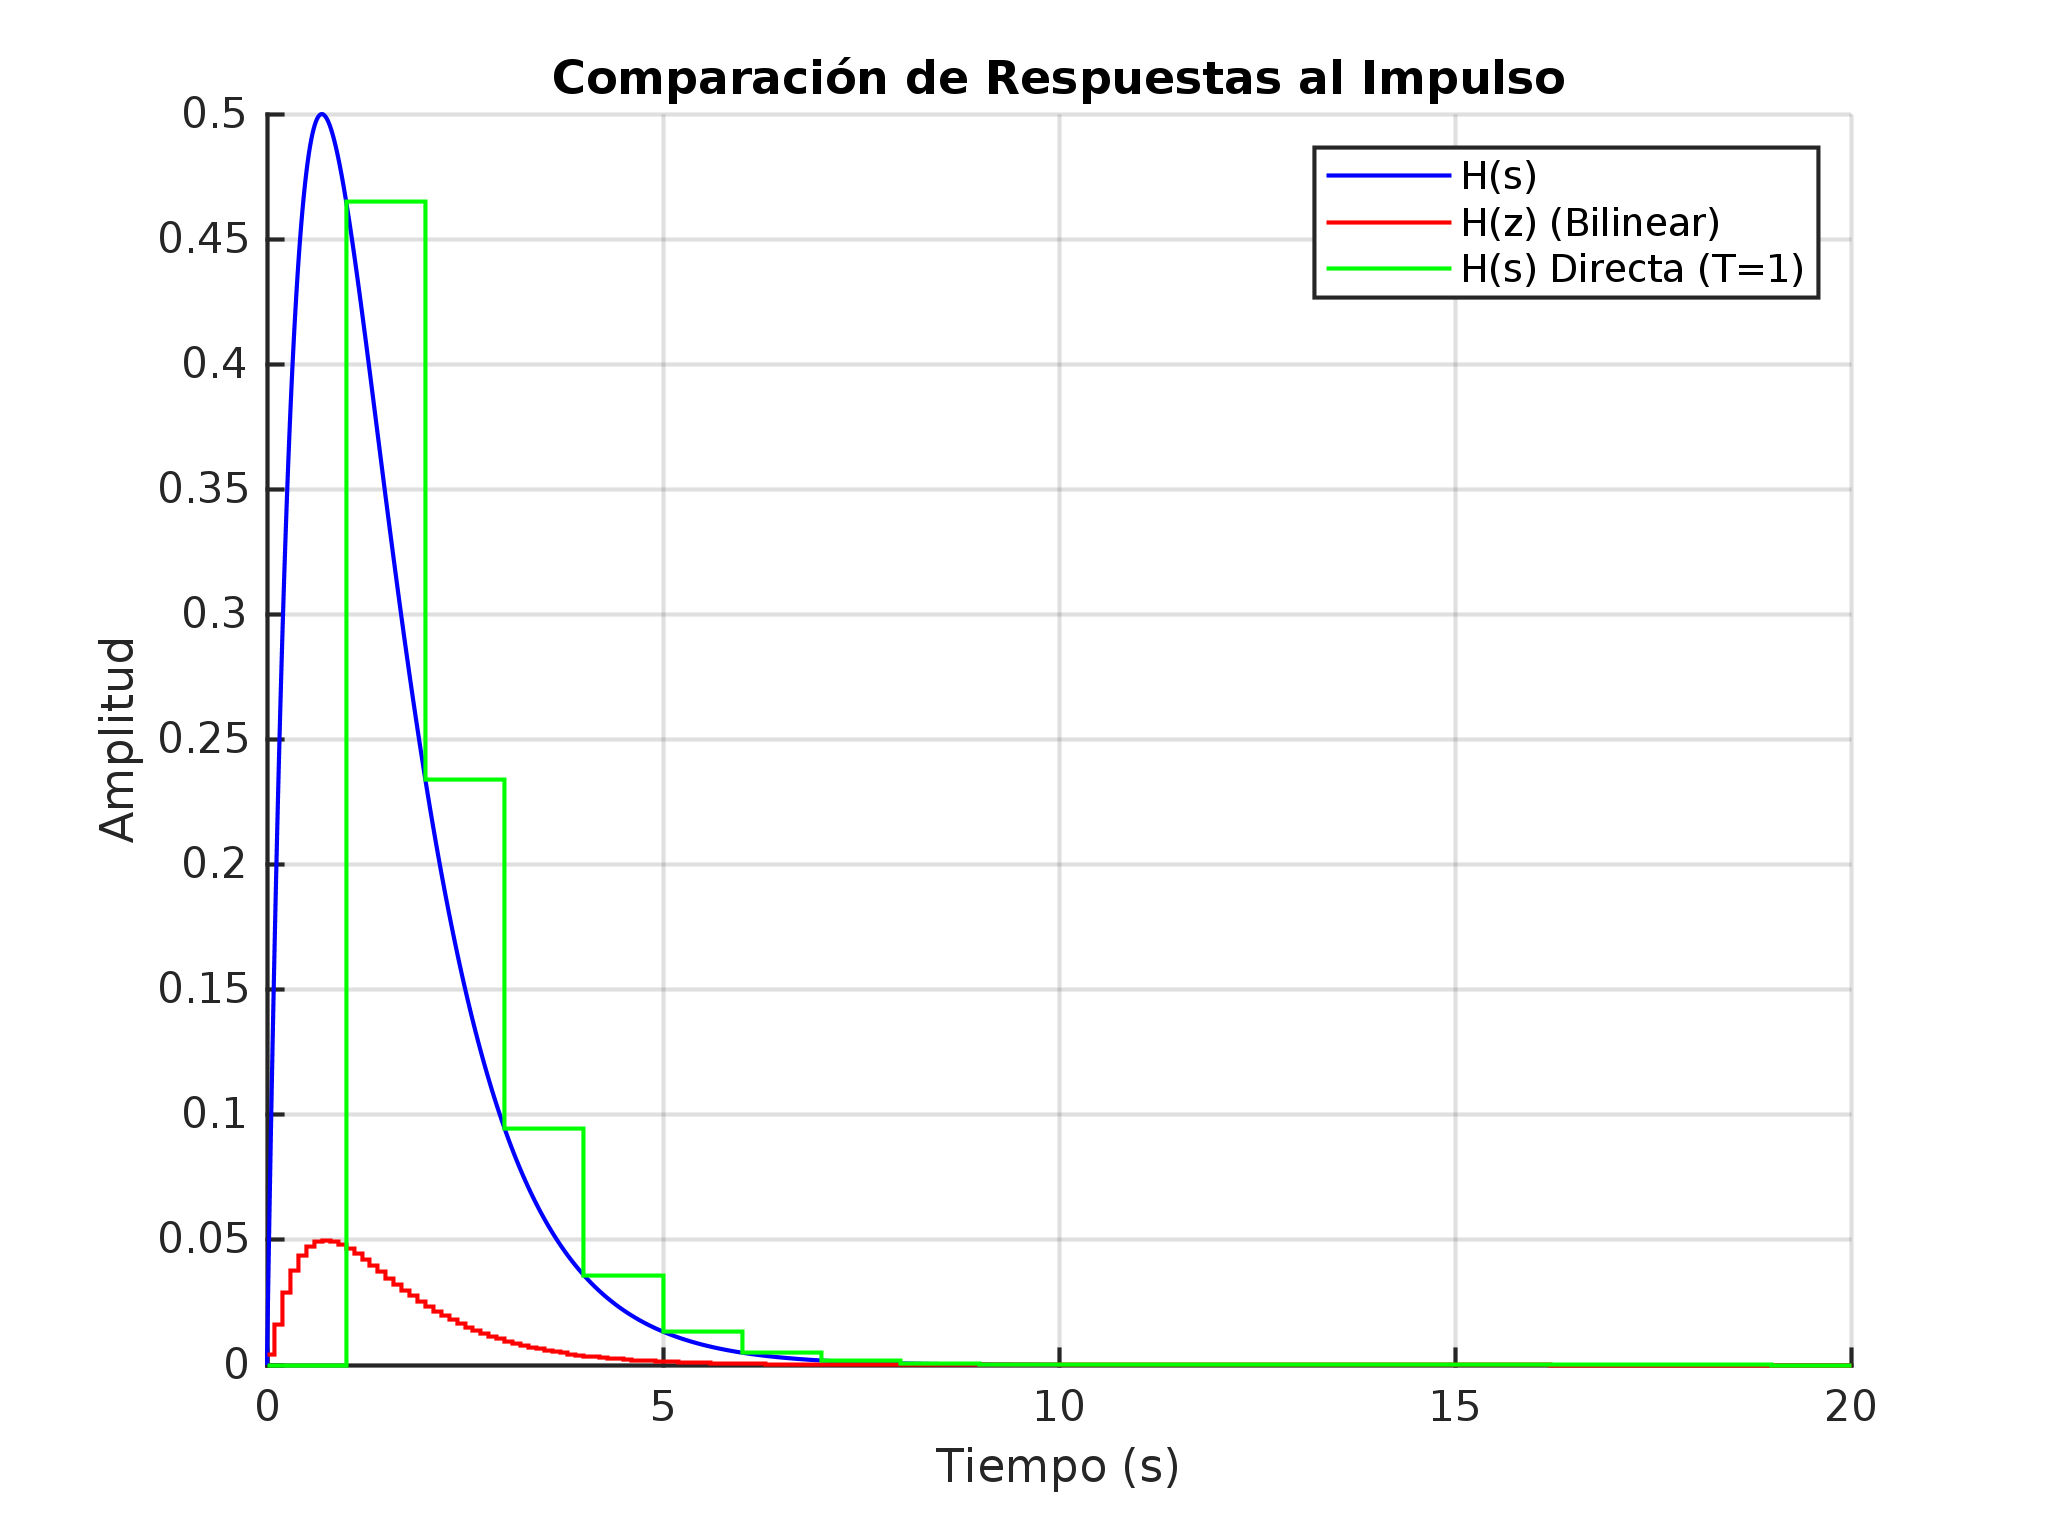
\includegraphics[width=1\textwidth]{./images/image1.png}
                \end{figure}

                Como se observa, la transformacion bilineal sufre alteraciones en la amplitud. Multiplicando por 10
                cada valor de amplitud, nos queda un grafico como el siguiente:
                \begin{figure}[h]
                    \centering
                    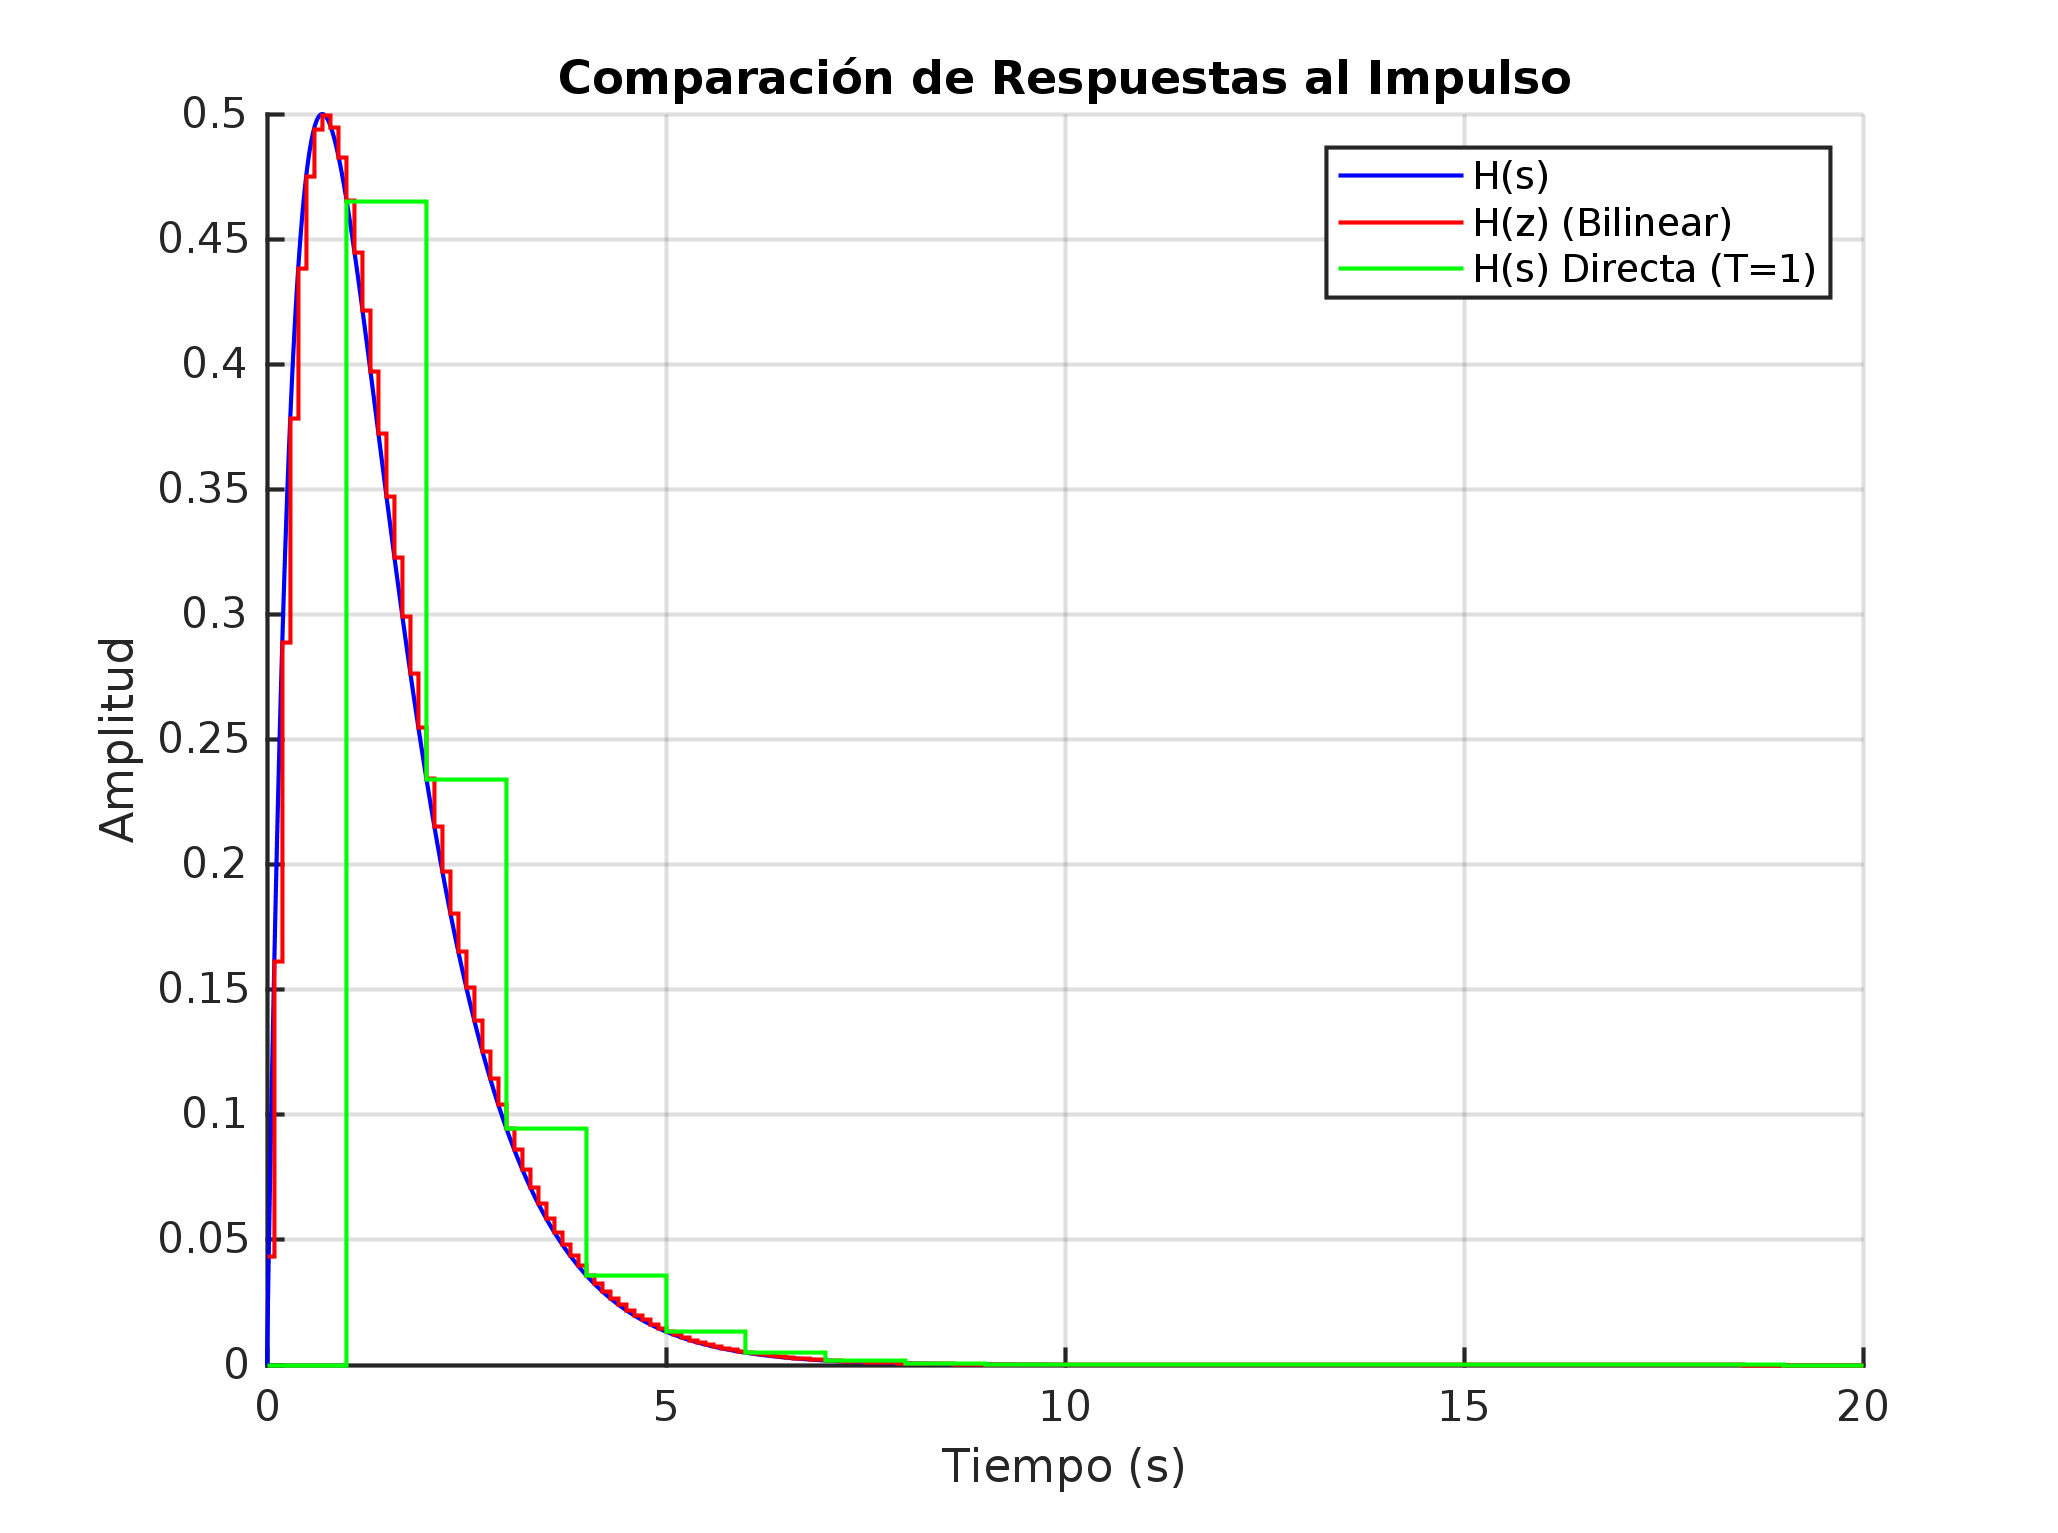
\includegraphics[width=1\textwidth]{./images/image2.png}
                \end{figure}

            \item \fs{} Obtener la $H_{(z)}$.\\

            \item \fs{} Desarrollar la respuesta $h_{[n]}$ al impulso $\delta_{[n]}$ por medio de la transformada Z.\\

            \item \fs{} Desarrollar la respuesta $\mu_{[n]}$ al impulso $y_{[n]}$ por medio de la transformada Z.\\

            \item \fs{} Verificar el TVI y TVF para ambas respuestas en ambos dominios.\\

            \item \fs{} Comparar graficamente las respuestas en tiempo continuo y tiempo discreto.\\

            \item \fs{} Comparar los TVI y TVF para ambas respuestas, continua y discreta.\\

            \item \fs{} Bosquejar el diagrama de BODE correspondiente para los dos filtros, y determimar $\omega_c$
                del filtro.\\

            \item \fs{} De acuerdo a los resultados obtenidos, ¿Que tipo de filtro es?\\

        \end{enumerate}

\end{document}
